%! Author = Leonhard Gahr <leonhard.gahr@gmail.com>
%! Date = 22/01/20
%! Info = Tx000_template

\chapter{Grundlagen - das MES Portal}
Um \gls{OP EX PH} zu steuern, werden viele Tools mitgeliefert, die unterschiedliche Funktionen erfüllen, z. B. das Anlegen neuer \glspl{PI} oder Starten von Arbeitsaufträgen. Manche Abläufe sind dabei so komplex, dass sie das Verwenden von mehreren Tools voraussetzen, die jeweils eine Authentifizierung erfordern und es müssen immer dieselben Abläufe ausgeführt werden. Für diese Aktivitäten wurde das MES Portal eingeführt, um solch grundlegende Arbeitsabläufe zu vereinfachen und teilweise zu automatisieren.\\
\Cref{fig-mes_portal_overview} zeigt eine reduzierte Version des Hauptmenüs des MES Portals. Hier ist u. a. das Modul Test Manager zu erkennen (\Cref{sec-test_manager}).

\begin{figure}[htbp]
  \centering
  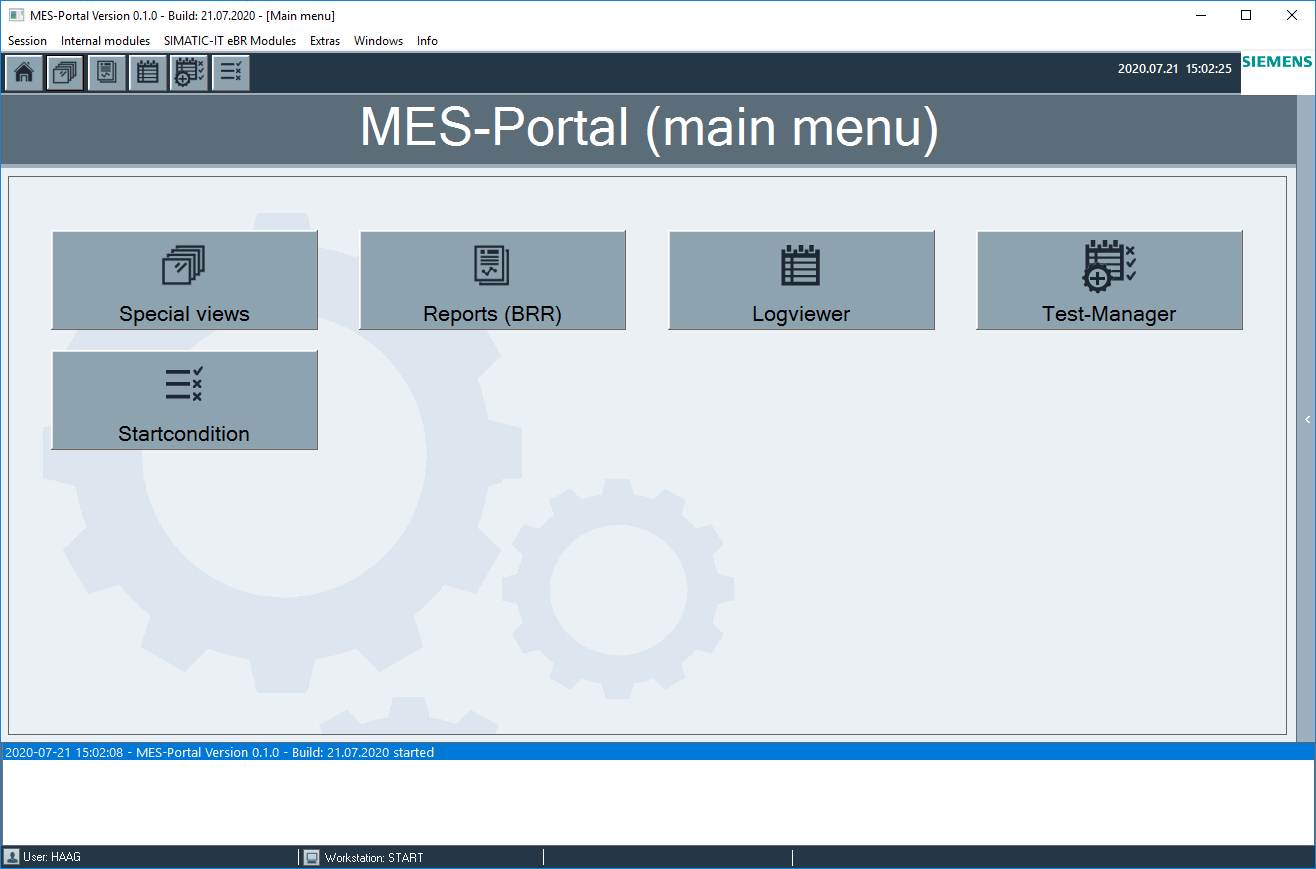
\includegraphics[width=.7\textwidth]{img/mes-portal_overview}
  \caption{\label{fig-mes_portal_overview}MES Portal - Hauptmenü}
\end{figure}

\section{Test Manager}\label{sec-test_manager}
Der Test Manager (\Cref{fig-mes_portal_test-manager}) bietet Funktionen zum automatisierten Testen von \glspl{PI}. Dabei werden die Funktionen unterteilt in \textbf{\nameref{sub_sec-test_manager-basics}}, die dem eigentlichen Ziel, dem Testen von Arbeitsaufträgen, dienen und \textbf{\nameref{sub_sec-test_manager-advanced}}, die der Benutzerfreundlichkeit dienen und das Verwenden des Test Managers erleichtern.

\begin{figure}[htbp]
  \centering
  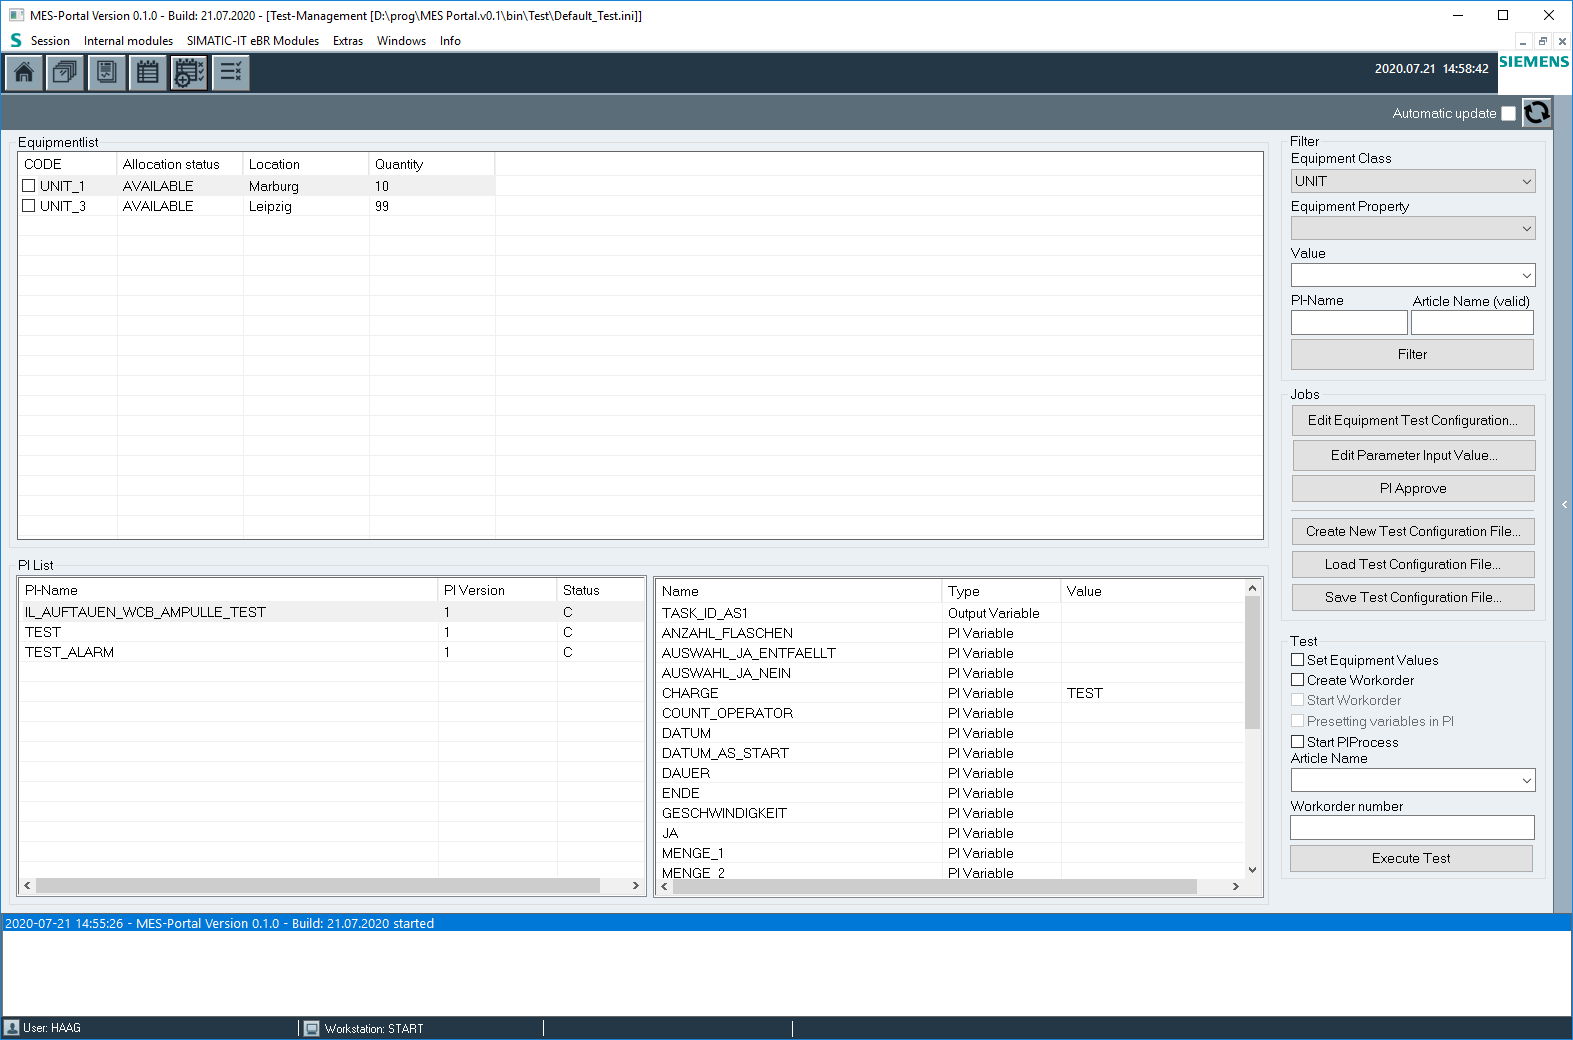
\includegraphics[width=\textwidth]{img/mes-portal_test-manage}
  \caption{\label{fig-mes_portal_test-manager}MES Portal - Test Manager (alt)}
\end{figure}

\newpage\subsection{Unterschied PI und Arbeitsauftrag}
Im Zusammenhang mit dem Test Manager kommen die Begriffe \gls{PI} und Arbeitsauftrag oft eng zusammen vor. Der Unterschied liegt in der Herkunft. Eine \gls{PI} wird von einem Nutzer definiert und beschreibt bestimmte Arbeitsschritte (\glsentrylong{PI}) auf einer konstanten Basis. Eine \gls{PI} wird im Allgemeinen nicht verändert.\\
Ein Arbeitsauftrag hingegen ist die ausführende Instanz einer \gls{PI}. Dieses Verhältnis ist äquivalent mit einem Objekt in der Objektorientierten Programmierung zu seiner Instanz. Eine \gls{PI} ist die Definition des Objekts und ein Arbeitsauftrag ist eine von womöglich vielen Instanzen dieses Objekts.\\
Wie ein Objekt auch kann eine \gls{PI} Variablen besitzen, die bei der Ausführung des Arbeitsauftrages gesetzt werden.

\subsection{Grundfunktionen}\label{sub_sec-test_manager-basics}
Dabei besteht der Prozess aus fünf Schritten:
\begin{enumerate}
\item Equipment Variablen setzen
\item Arbeitsauftrag erstellen
\item Arbeitsauftrag starten
\item \gls{PI} Variablen setzen
\item PIProcess starten
\end{enumerate}

\subsubsection{Equipment Variablen setzen}
In diesem Schritt werden die konfigurierten Werte für die Equipments in die Datenbank geschrieben, auf die der Arbeitsauftrag später zugreifen wird.

\subsubsection{Arbeitsauftrag erstellen}
Hier wird über die Schnittstelle zu \gls{OP EX PH} ein Arbeitsauftrag mit einer gegebenen Arbeitsauftragsnummer im System angelegt.

\subsubsection{Arbeitsauftrag starten}
Der erstellte Arbeitsauftrag wird gestartet.

\subsubsection{PI Variablen setzen}
Die konfigurierten Variablen werden in der Datenbank zu dem Arbeitsauftrag hinzugefügt.

\subsubsection{PIProcess starten}
Startet das Programm PIProcess, mit dem der Arbeitsauftrag überwacht werden kann und ggf. manuelle Eingaben getätigt werden können.

\subsection{Zusatzfunktionen}\label{sub_sec-test_manager-advanced}
Die Zusatzfunktionen des Test Managers bestehen aus den Kategorien \textbf{Filter} und \textbf{Jobs}, die sich auf der rechten Seite der \Cref{fig-mes_portal_test-manager} befinden.

\subsubsection{Filter}
Die Filter beziehen sich teilweise auf die Equipments, aber auch auf die \glspl{PI}.\\
Equipments können nach der Klasse gefiltert werden. Die Klasse ist ein Bezeichner für die Art des Equipments (z. B. eine Maschine). Außerdem besitzen Equipments Eigenschaften in der Datenbank (z. B. \enquote{Allocation Status} oder Standort). Nach diesen Eigenschaften kann ebenfalls gefiltert werden.\\
\glspl{PI} können nach Namen oder nach dem Produkt gefiltert werden, das sie produzieren.

\subsubsection{Jobs}
Unter der Kategorie Jobs befinden sich einige Funktionen, die die Arbeit mit den einzelnen \glspl{PI} erleichtern. Die drei Knöpfe \enquote{Create New-}, \enquote{Load-} und \enquote{Save Test Configuration...} dienen dem Speichern der aktuellen Einstellungen, um die Arbeit an der jeweiligen \gls{PI} wieder aufnehmen zu können.\\
Die Funktionen \enquote{Edit Equipment Test Configuration...} und \enquote{Edit Parameter Input Value...} öffnen jeweils einen Dialog, in dem die Werte für alle aktuell sichtbaren Equipments bzw. \gls{PI}-Variablen auf einmal gesetzt werden können. Mit \enquote{PI Approve} wird der Status der ausgewählten \gls{PI} auf \enquote{Approved} gesetzt, damit sie ausgeführt werden kann.

\newpage\section{Workorder Planner}
Um eine bessere Übersicht über geplante oder bereits abgeschlossene Arbeitsaufträge zu erhalten, zeigt der Workorder Planner alle existierenden Arbeitsaufträge in chronologischer Reihenfolge in einem Kalender an (\Cref{fig-mes_portal_workorder-planner}). Da mehrere Arbeitsaufträge gleichzeitig in \gls{OP EX PH} erfasst und ausgeführt werden können, werden die Aufträge nach der Anlage gruppiert, in der sie ausgeführt werden. In \gls{OP EX PH} werden Arbeitsaufträge ohne Gruppierung in einer Tabelle angezeigt, die keine gute Übersicht über Start- und Endzeitpunkt aller Arbeitsaufträge gibt, um z. B. die Auslastung einer Produktionsanlage einsehen zu können.
\begin{figure}[htbp]
  \centering
  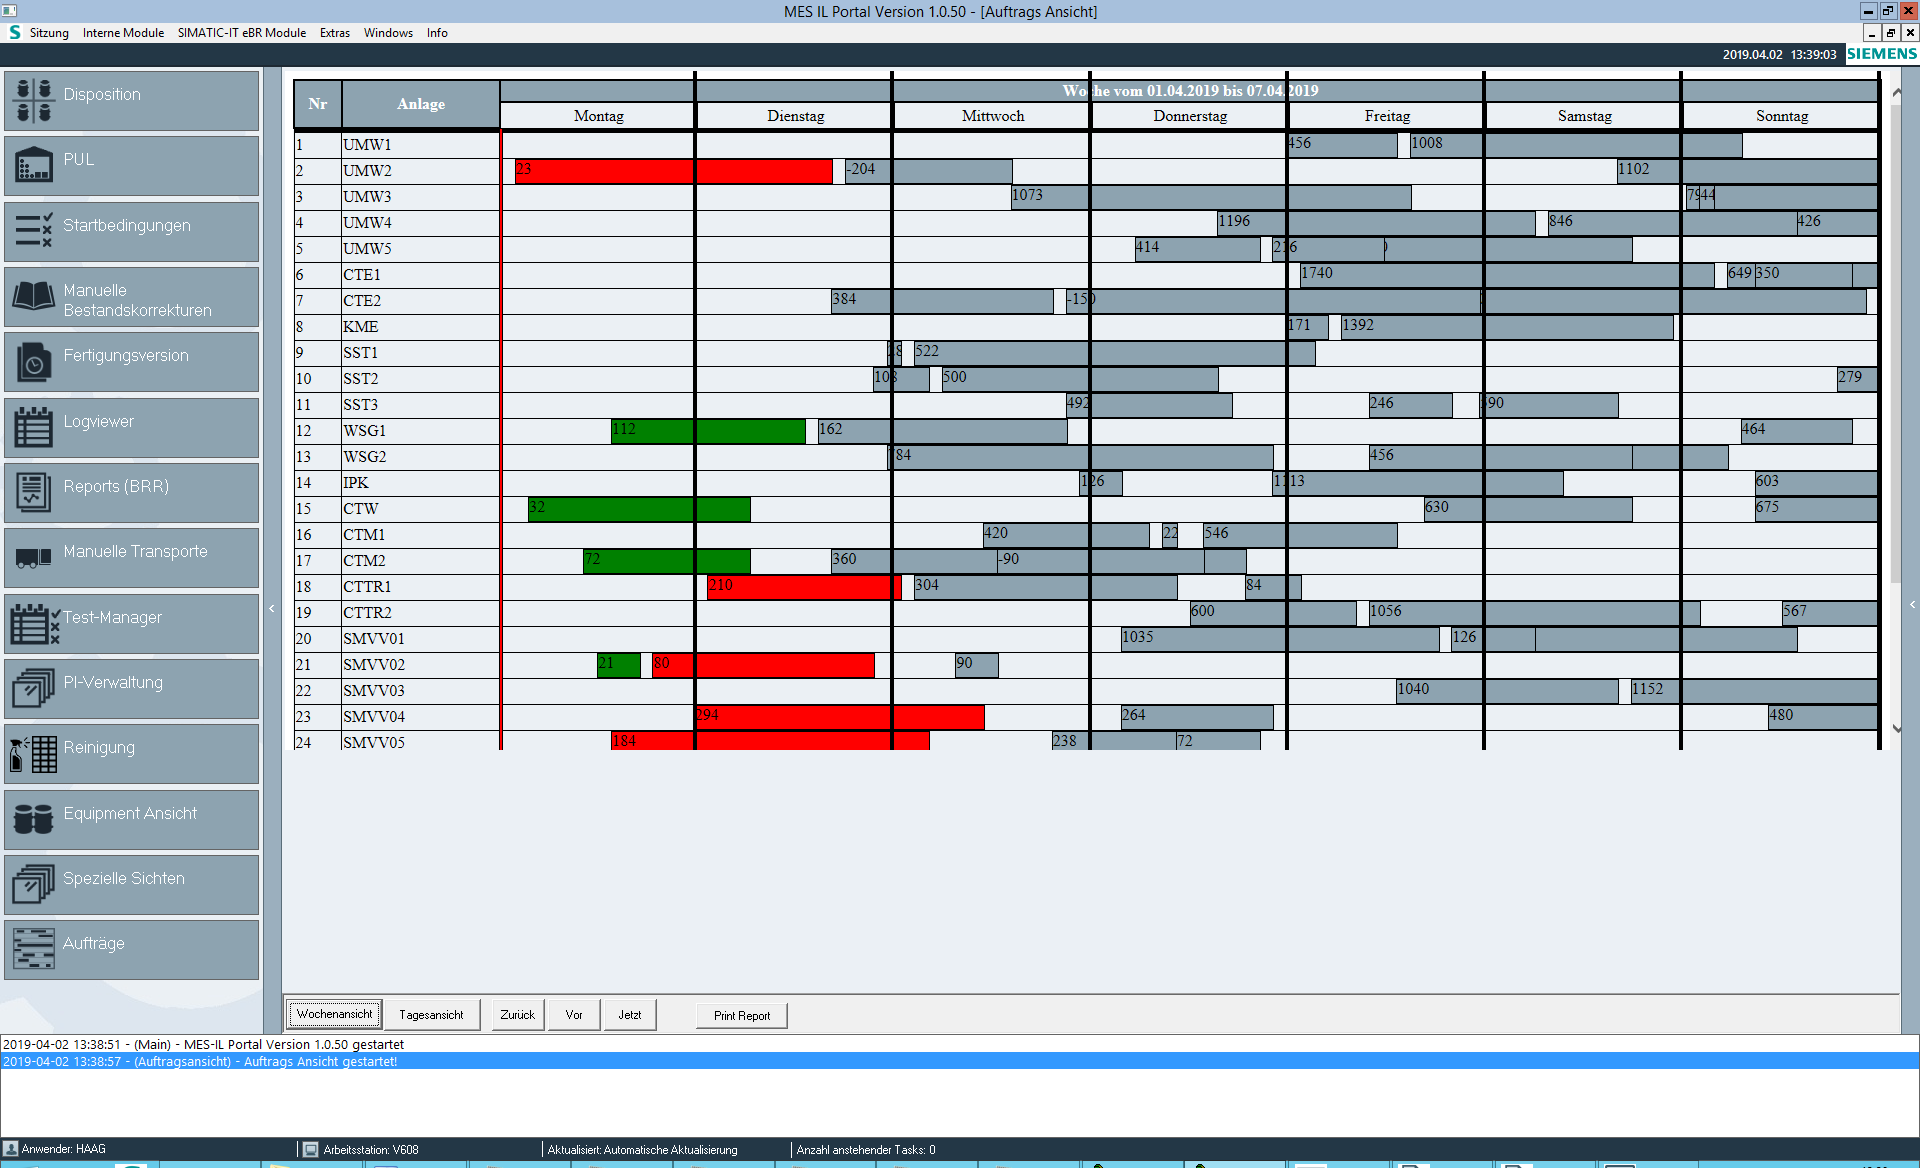
\includegraphics[width=\textwidth]{img/mes-portal_workorder-planner}
  \caption{\label{fig-mes_portal_workorder-planner}MES Portal - Workorder Planner (alt)}
\end{figure}

\noindent Die angezeigten Daten zu den Arbeitsaufträgen werden aus der \gls{OP EX PH} Datenbank bezogen. In dieser Datenbank werden jedoch keine Daten zum geschätzten Abschlusszeitpunkt eines Arbeitsauftrages abgelegt. Diese Daten kommen aus einem System von SAP, das diese Information in der Datenbank in einem benutzerdefinierten Feld \enquote{XFIELD09} einträgt. Die \enquote{XFields} sind zehn durchnummerierte, standardmäßig leere Spalten zu jedem Arbeitsauftrag in der Datenbank.